\documentclass{beamer}
\usepackage[T1]{fontenc}
\usepackage[utf8]{inputenc}
\usepackage{amsmath}
\usepackage{amsfonts}
\usepackage{amsthm}
\usepackage{array}
\usepackage{graphicx}
\usepackage{listings}
\usepackage{color}
\usepackage{fancyhdr}
\usepackage{tikz}
\usetikzlibrary{calc,shapes.multipart,chains,arrows}
\usepackage{float}
\usepackage{caption}
\usepackage[linguistics]{forest}
\usepackage[cache=false]{minted}
\usemintedstyle{default}
\newminted{haskell}{}
\graphicspath{{./images/}}
\setbeamertemplate{frametitle}{%
  \usebeamerfont{frametitle}\insertframetitle%
  \vphantom{g}% To avoid fluctuations per frame
  % \hrule% Uncomment to see desired effect, without a full-width hrule
  \par\hspace*{-\dimexpr0.5\paperwidth-0.5\textwidth}\rule[0.5\baselineskip]{\paperwidth}{0.4pt}
  \par\vspace*{-\baselineskip}% <-- reduce vertical space after rule
}

\usetheme{Boadilla}
\title{Analysis on Random Access Zippers}

\author{Juan Pablo Royo Sales}
\institute{Universitat Politècnica de Catalunya}
\date{June $11^{th}$, 2020}
\begin{document}

\begin{frame}
\titlepage
\end{frame}

\begin{frame}{Agenda}
  \tableofcontents
\end{frame}

\begin{frame}{Agenda}
  \section{Spoiler}
  \tableofcontents[currentsection]
\end{frame}

\begin{frame}[fragile]{Spoiler}

  \begin{block}{Paper}
    \begin{itemize}
      \item Based on \textbf{Headley, Kyle and Hammer, Matthew. (2016). The Random Access Zipper: Simple, Purely-Functional Sequences.}
    \end{itemize}
  \end{block}

\end{frame}

\begin{frame}[fragile]{Spoiler}

  \begin{block}{Paper}
    \begin{itemize}
      \item Based on \textbf{Headley, Kyle and Hammer, Matthew. (2016). The Random Access Zipper: Simple, Purely-Functional Sequences.}
      \item Combines \textbf{Zippers} and \textbf{Probabilistic Balanced Binary Tree (PBBT)}
    \end{itemize}
  \end{block}

\end{frame}


\begin{frame}[fragile]{Spoiler}

  \begin{block}{Paper}
    \begin{itemize}
      \item Based on \textbf{Headley, Kyle and Hammer, Matthew. (2016). The Random Access Zipper: Simple, Purely-Functional Sequences.}
      \item Combines \textbf{Zippers} and \textbf{Probabilistic Balanced Binary Tree (PBBT)}
      \item \textbf{Summary of the Paper}
        \begin{itemize}
            \item Definition of Data Structure
            \item Implementation in \textbf{OCaml}
            \item Experiments to probe some claims
        \end{itemize}
    \end{itemize}
  \end{block}

\end{frame}

\begin{frame}[fragile]{Spoiler}

  \begin{block}{Paper}
    \begin{itemize}
      \item Based on \textbf{Headley, Kyle and Hammer, Matthew. (2016). The Random Access Zipper: Simple, Purely-Functional Sequences.}
      \item Combines \textbf{Zippers} and \textbf{Probabilistic Balanced Binary Tree (PBBT)}
      \item \textbf{Summary of the Paper}
        \begin{itemize}
            \item Definition of Data Structure
            \item Implementation in \textbf{OCaml}
            \item Experiments to probe some claims
        \end{itemize}
    \end{itemize}
  \end{block}

    \begin{block}{My Work}
    \begin{itemize}
      \item Analyze the paper
      \item \textbf{Haskell} Implementation
      \item Reproduce Experiments
    \end{itemize}
  \end{block}

\end{frame}

\begin{frame}{Agenda}
  \section{Zippers}
  \tableofcontents[currentsection]
\end{frame}


\begin{frame}[fragile]{Zippers}

  \begin{block}{Why do I choose this structure?}
    \begin{itemize}
      \item Interested on Zippers as \textbf{FP} Data Structure
    \end{itemize}
  \end{block}

\end{frame}

\begin{frame}[fragile]{Zippers}

  \begin{block}{Why do I choose this structure?}
    \begin{itemize}
      \item Interested on Zippers as \textbf{FP} Data Structure
      \item Type Level correspondence with Derivatives - \textbf{Math reasoning!!!}\footnote{Mcbride, Conor. (2009). The Derivative of a Regular Type is its Type of One-Hole Contexts (Extended Abstract).}
    \end{itemize}
  \end{block}

\end{frame}

\begin{frame}[fragile]{Zippers}

 \begin{block}{Zipper}

  \begin{minipage}[t]{\linewidth}
    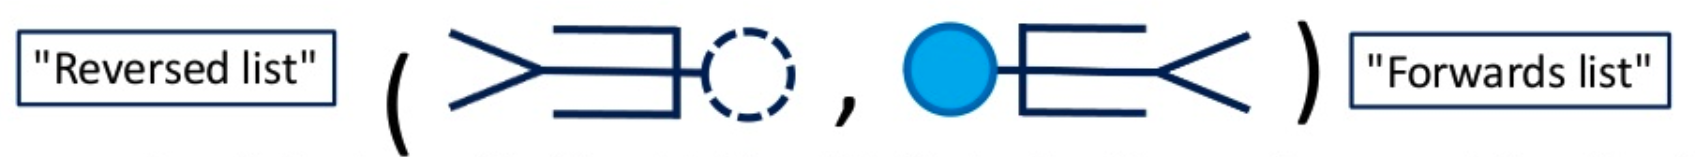
\includegraphics[width=\textwidth]{zipper_1}
  \end{minipage}

  \begin{minted}[escapeinside=||]{haskell}
    type Zipper a = ([a], [a])

    goLeft :: Zipper a -> Zipper a
    goLeft (|\colorbox{red}{\textbf{x}}| : xs, ys) = ( xs, |\colorbox{red}{\textbf{x}}| : ys )

    goRight :: Zipper a -> Zipper a
    goRight (xs, |\colorbox{red}{\textbf{y}}| : ys) = ( |\colorbox{red}{\textbf{y}}| : xs, ys )
  \end{minted}


\end{block}

\end{frame}

\begin{frame}[fragile]{Zippers}

 \begin{block}{Zipper}

  \begin{minipage}[t]{\linewidth}
    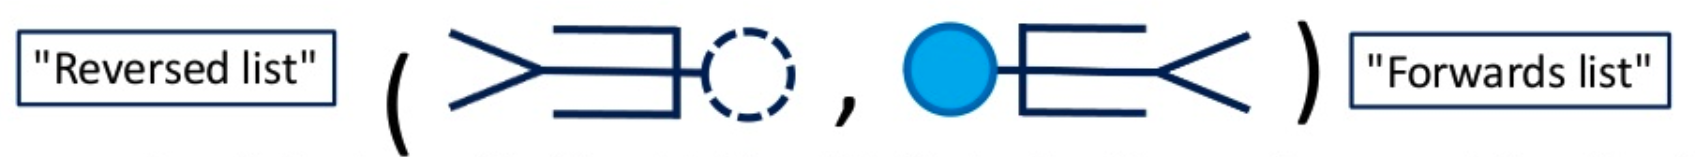
\includegraphics[width=\textwidth]{zipper_1}
  \end{minipage}

  \begin{minted}[escapeinside=||]{haskell}
    type Zipper a = ([a], [a])

    goLeft :: Zipper a -> Zipper a
    goLeft (|\colorbox{red}{\textbf{x}}| : xs, ys) = ( xs, |\colorbox{red}{\textbf{x}}| : ys )

    goRight :: Zipper a -> Zipper a
    goRight (xs, |\colorbox{red}{\textbf{y}}| : ys) = ( |\colorbox{red}{\textbf{y}}| : xs, ys )
  \end{minted}


\end{block}

\begin{block}{Hints}
  Enable \textbf{$O(1)$} time for update and remove elements which in regular \mintinline{haskell}{List} in pure \textbf{FP} is worst-case $O(n)$
\end{block}
\end{frame}

\begin{frame}{Agenda}
  \section{RAZ - Structure and Features}
  \tableofcontents[currentsection]
\end{frame}

\begin{frame}[fragile]{RAZ - Structure and Features}

  \begin{block}{RAZ - Random Access Zippers}
    \begin{itemize}
      \item Combines \textbf{Zipper} with \textbf{PBBT}
      \item Focuses on \textit{Sequence} like structures
      \item \textbf{Edition:} $O(1)$ -- \textbf{Random Access Elements:} $O(\log{n})$ Amortized
    \end{itemize}
  \end{block}

\end{frame}

\begin{frame}[fragile]{RAZ - Structure and Features}

  \begin{block}{RAZ - Random Access Zippers}
    \begin{itemize}
      \item Combines \textbf{Zipper} with \textbf{PBBT}
      \item Focuses on \textit{Sequence} like structures
      \item \textbf{Edition:} $O(1)$ -- \textbf{Random Access Elements:} $O(\log{n})$ Amortized
    \end{itemize}
  \end{block}

   \begin{block}{Author's Motivation}
    \begin{itemize}
      \item \textbf{FP} \textit{Sequence} like structure has inefficient \textbf{access} and \textbf{edit} costs. $O(n)$ worst case
      \item \textbf{Finger-Trees} and \textbf{RRB-Vectors (Relaxed Radix Balanced Vectors)} overcome this but are complex and not extensible as \mintinline{haskell}{List}.
    \end{itemize}
  \end{block}

\end{frame}

\begin{frame}[fragile]{RAZ - Structure and Features}

  \begin{block}{RAZ - Random Access Zippers}
    \begin{itemize}
      \item Combines \textbf{Zipper} with \textbf{PBBT}
      \item Focuses on \textit{Sequence} like structures
      \item \textbf{Edition:} $O(1)$ -- \textbf{Random Access Elements:} $O(\log{n})$ Amortized
    \end{itemize}
  \end{block}

   \begin{block}{Author's Motivation}
    \begin{itemize}
      \item \textbf{FP} \textit{Sequence} like structure has inefficient \textbf{access} and \textbf{edit} costs. $O(n)$ worst case
      \item \textbf{Finger-Trees} and \textbf{RRB-Vectors (Relaxed Radix Balanced Vectors)} overcome this but are complex and not extensible as \mintinline{haskell}{List}.
    \end{itemize}
  \end{block}

   \begin{block}{RAZ Goal}
    \begin{itemize}
      \item Same costs as \textbf{Finger-Trees} and \textbf{RRB-Vectors}
      \item \mintinline{haskell}{List} interface and extensible.
    \end{itemize}
  \end{block}

\end{frame}


\begin{frame}[fragile]{RAZ - Structure and Features}
  \begin{block}{RAZ - Internals}
   \begin{minipage}[t]{\linewidth}
     \begin{center}
      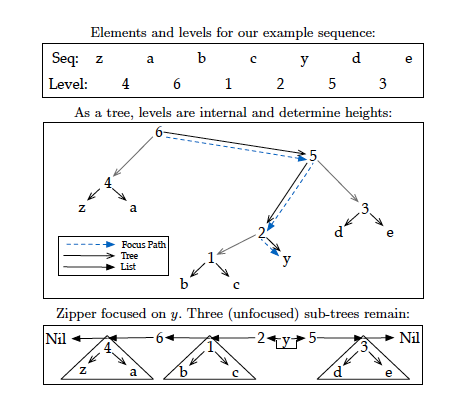
\includegraphics[scale=0.5]{raz_1}
     \end{center}
   \end{minipage}
 \end{block}
\end{frame}

\begin{frame}[fragile]{RAZ - Structure and Features}

  \begin{block}{RAZ - Internals}
    \begin{itemize}
      \item Switch between 2 estructure
      \item \textbf{Zipper}: Power of \textbf{cursor} for focusing and navigation
      \item \textbf{PBBT}: Using a Negative Binomial Distribution to build a \textbf{Balanced Tree} and has fast random access to any element.
    \end{itemize}
  \end{block}

\end{frame}

\begin{frame}[fragile]{RAZ - Structure and Features}

  \begin{block}{RAZ - Costs}
    \begin{table}[H]
 \begin{tabular}{|l|l|}
  \hline
   Function:: Type & Time Complexity\\
  \hline
  \mintinline{haskell}{focus :: Int -> Tree a -> Raz a} & $O(\log{n})$ expected \\
  \mintinline{haskell}{unfocus :: Raz a -> Tree a} & $O(\log{n} + m \times \log^2{m})$ expected \\
  \hline
  \multicolumn{1}{|p{3cm}|}{\setlength{\rightskip}{0pt plus 1 fill}\mintinline[breaklines]{haskell}{insert :: RandomGen g => g -> Dir -> a -> Raz a -> (Raz a, g)}} & $O(1)$ worst-case \\
  \hline
  \mintinline{haskell}{remove :: Dir -> Raz a -> Raz a} & $O(1)$ amortized  \\
  \mintinline{haskell}{replaceC :: a -> Raz a -> Raz a} & $O(1)$ worst-case  \\
  \mintinline{haskell}{move :: Dir -> Raz a -> Raz a} & $O(1)$ amortized  \\
  \mintinline{haskell}{viewC :: Raz a -> a} & $O(1)$ worst-case  \\
  \hline
 \end{tabular}
\end{table}


  \end{block}

\end{frame}

\begin{frame}
  \frametitle{Agenda}
  \section{Haskell Implementation}
  \tableofcontents[currentsection]
\end{frame}

\begin{frame}[fragile]{Haskell Implementation}

  \begin{minted}[fontsize=\tiny]{haskell}
    type NLev = Int

    type Cnt = Int

    data Dir
      = L
      | R
      deriving (Eq, Show, Ord)

    data Tree a
      = Empty
      | Leaf a
      | Bin !NLev !Cnt !(Tree a) !(Tree a)
      deriving (Functor, Foldable, Traversable)

    data TList a
      = Nil
      | Cons a !(TList a)
      | Level !NLev !(TList a)
      | LTree !(Tree a) !(TList a)
      deriving (Functor, Foldable, Traversable)

    type Raz a = (TList a, a, TList a)
  \end{minted}

\end{frame}

\begin{frame}[fragile]{Haskell Implementation}

  \begin{minted}[fontsize=\tiny,highlightlines={1-3}]{haskell}
    type NLev = Int  -- Level of the Tree

    type Cnt = Int  -- Keep Counter elements in the Tree

    data Dir
      = L
      | R
      deriving (Eq, Show, Ord)

    data Tree a
      = Empty
      | Leaf a
      | Bin !NLev !Cnt !(Tree a) !(Tree a)
      deriving (Functor, Foldable, Traversable)

    data TList a
      = Nil
      | Cons a !(TList a)
      | Level !NLev !(TList a)
      | LTree !(Tree a) !(TList a)
      deriving (Functor, Foldable, Traversable)

    type Raz a = (TList a, a, TList a)
  \end{minted}

\end{frame}


\begin{frame}[fragile]{Haskell Implementation}

  \begin{minted}[fontsize=\tiny,highlightlines={5-8}]{haskell}
    type NLev = Int

    type Cnt = Int

    data Dir        -- Direction. Go to Left 'L' or Go to Right 'R'
      = L
      | R
      deriving (Eq, Show, Ord)

    data Tree a
      = Empty
      | Leaf a
      | Bin !NLev !Cnt !(Tree a) !(Tree a)
      deriving (Functor, Foldable, Traversable)

    data TList a
      = Nil
      | Cons a !(TList a)
      | Level !NLev !(TList a)
      | LTree !(Tree a) !(TList a)
      deriving (Functor, Foldable, Traversable)

    type Raz a = (TList a, a, TList a)
  \end{minted}

\end{frame}

\begin{frame}[fragile]{Haskell Implementation}

  \begin{minted}[fontsize=\tiny,highlightlines={10-14}]{haskell}
    type NLev = Int

    type Cnt = Int

    data Dir
      = L
      | R
      deriving (Eq, Show, Ord)

    data Tree a  -- Tree for Random access
      = Empty    -- Empty Node
      | Leaf a   -- Leaf
      | Bin !NLev !Cnt   !(Tree a)         !(Tree a)
        --  ^ Node ----      ^ Left Tree       ^ Right Tree
      deriving (Functor, Foldable, Traversable)

    data TList a
      = Nil
      | Cons a !(TList a)
      | Level !NLev !(TList a)
      | LTree !(Tree a) !(TList a)
      deriving (Functor, Foldable, Traversable)

    type Raz a = (TList a, a, TList a)
  \end{minted}

\end{frame}

\begin{frame}[fragile]{Haskell Implementation}

  \begin{minted}[fontsize=\tiny,highlightlines={17-27}]{haskell}
    type NLev = Int

    type Cnt = Int

    data Dir
      = L
      | R
      deriving (Eq, Show, Ord)

    data Tree a
      = Empty
      | Leaf a
      | Bin !NLev !Cnt !(Tree a) !(Tree a)
      deriving (Functor, Foldable, Traversable)

    data TList a
      = Nil  -- Empty
      | Cons   a      !(TList a)
        --  ^ Elem      ^ Linked List after element
      | Level !NLev !(TList a)
            -- ^ Level  ^ List
      | LTree !(Tree a) !(TList a)
            --  ^ Tree    ^ List
      deriving (Functor, Foldable, Traversable)

    type Raz a = (TList a, a, TList a)
              -- ^ Zipper
  \end{minted}
\end{frame}

\begin{frame}[fragile]{Haskell Implementation}

  \begin{block}{Some combinators}

\begin{listing}[H]
  \inputminted[firstline=90, lastline=91, breaklines, fontsize=\tiny]{haskell}{../src/Data/Zipper/Random.hs}
  \inputminted[firstline=104, lastline=105, breaklines, fontsize=\tiny]{haskell}{../src/Data/Zipper/Random.hs}
  \inputminted[firstline=122, lastline=129, breaklines, fontsize=\tiny]{haskell}{../src/Data/Zipper/Random.hs}
  \inputminted[firstline=132, lastline=136, breaklines, fontsize=\tiny]{haskell}{../src/Data/Zipper/Random.hs}
\end{listing}


\end{block}

\end{frame}


\begin{frame}
  \frametitle{Agenda}
  \section{Experiments Reproduction}
  \tableofcontents[currentsection]
\end{frame}

\begin{frame}[fragile]{Experiments Reproduction}

  \begin{block}{\textbf{RAZ} vs. \textbf{Finger-Tree}}
    \begin{itemize}
      \item \textbf{Experiment 1} Building time with different amount of elements until building a structure with $1M$
      \item \textbf{Experiment 2} Inserting increasing amount of elements starting from $1M$ until reaching $100M$
      \end{itemize}
  \end{block}

\end{frame}

\begin{frame}[fragile]{Experiments Reproduction}

  \begin{block}{Experiment 1}
  \begin{figure}[!tbp]
  \centering
  \textbf{Authors' Results}\par\medskip
   \begin{minipage}[b]{0.4\textwidth}
     \begin{center}
      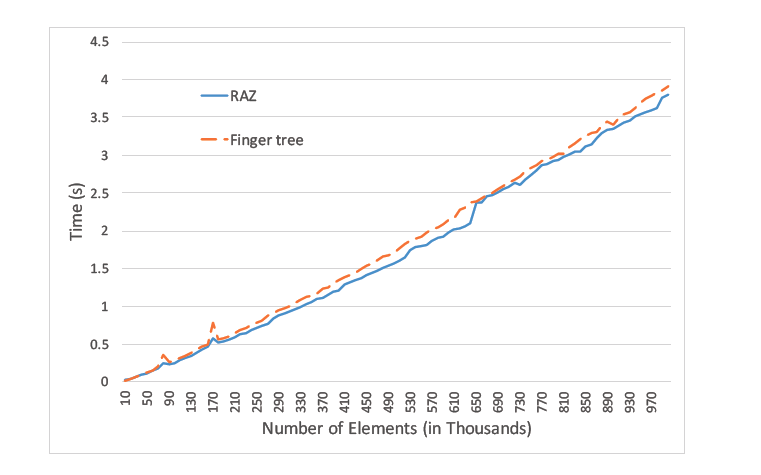
\includegraphics[width=\textwidth]{author_exp_1}
     \end{center}
  \end{minipage}

   \textbf{Haskell Impl Results}\par\medskip
    \begin{minipage}[b]{0.4\textwidth}
     \begin{center}
      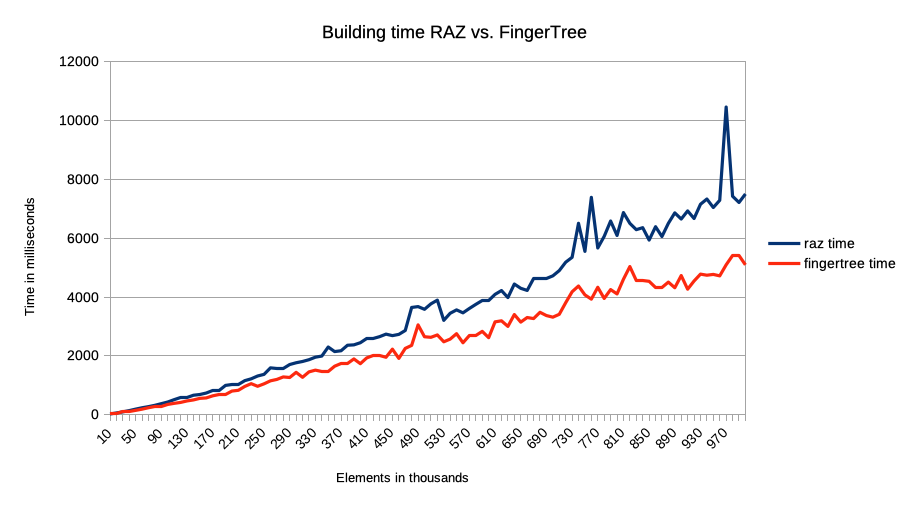
\includegraphics[width=\textwidth]{raz_ftree_exp_1}
     \end{center}
   \end{minipage}

 \end{figure}
  \end{block}

\end{frame}

\begin{frame}[fragile]{Experiments Reproduction}

  \begin{block}{Experiment 2}
  \begin{figure}[!tbp]
  \centering
  \textbf{Authors' Results}\par\medskip
   \begin{minipage}[b]{0.4\textwidth}
     \begin{center}
      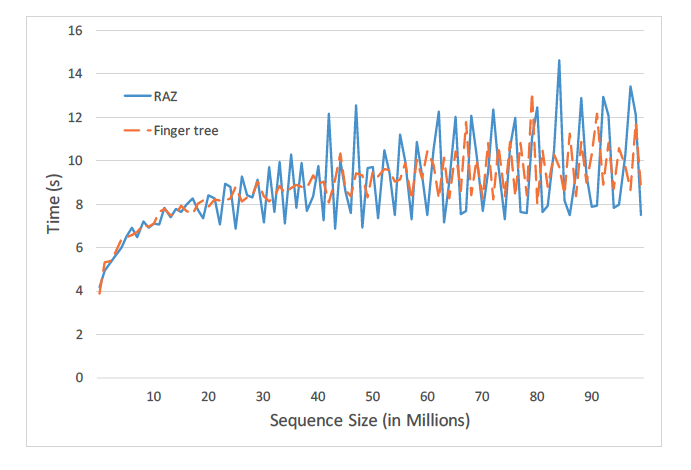
\includegraphics[width=\textwidth]{author_exp_2}
     \end{center}
  \end{minipage}

   \textbf{Haskell Impl Results}\par\medskip
    \begin{minipage}[b]{0.4\textwidth}
     \begin{center}
      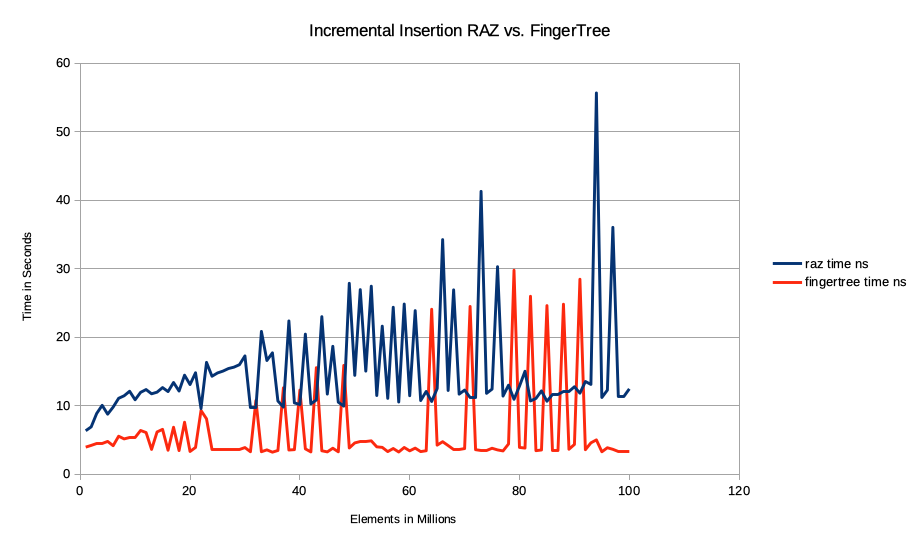
\includegraphics[width=\textwidth]{raz_ftree_exp_2}
     \end{center}
   \end{minipage}

 \end{figure}
  \end{block}

\end{frame}

\begin{frame}
  \frametitle{Agenda}
  \section{Benchmark}
  \tableofcontents[currentsection]
\end{frame}

\begin{frame}[fragile]{Benchmark}

  \begin{block}{Additionally done in this work}
   \begin{minipage}[t]{\linewidth}
    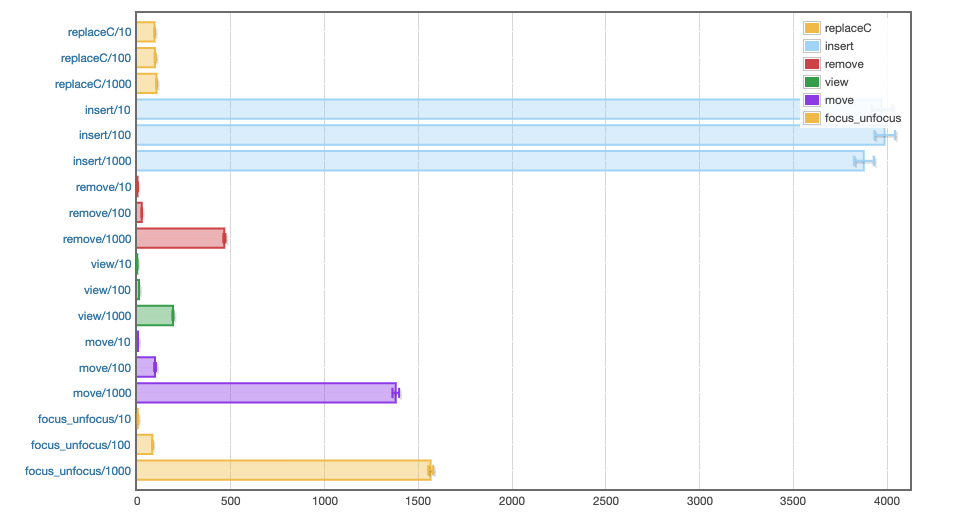
\includegraphics[width=\textwidth]{raz_bench}
  \end{minipage}

  \end{block}

\end{frame}




\begin{frame}
  \frametitle{Agenda}
  \section{Caveats and Analysis}
  \tableofcontents[currentsection]
\end{frame}

\begin{frame}[fragile]{Caveats and Analysis}

  \begin{block}{About Authors Work}
    \begin{itemize}
    \item \textbf{No rigorous Math} analysis is provided regarding costs
    \item Experiments are somehow biased by focusing and refocusing compared with split Finger Tree. No experiment or benchmark comparison with all combinators of the structure
    \item Both claims about the advantage of the structure cannot be conclusively seen after all.
    \item \textbf{Claim 1 - Same Performance as Finger Tree:} Not conclusive
    \item \textbf{Claim 2 - Extensibility and Simplicity:} There is nothing provided in the work about extension. Although implementation is simple some functionalities like \mintinline{haskell}{joinSides}, \mintinline{haskell}{trim}, \mintinline{haskell}{grow} are not so simple.
  \end{itemize}
  \end{block}

\end{frame}

\begin{frame}[fragile]{Caveats and Analysis}

  \begin{block}{About Haskell Implementation}
    \begin{itemize}
      \item A hard work needed to be done in order to reach that performance level.
      \item Difference between \textbf{Strict} and \textbf{Non Strict} evaluation makes the difference.
      \item Although a regular implementation of \textbf{Finger Tree} was used for comparison, it is still better than \textbf{RAZ}.
  \end{itemize}
  \end{block}

\end{frame}



\begin{frame}
  \frametitle{Agenda}
  \section{Conclusions}
  \tableofcontents[currentsection]
\end{frame}

\begin{frame}[fragile]{Conclusion}

    \begin{itemize}
      \item Quite efficient structure for \textbf{Sequence} like in \textbf{FP}
      \item It is not more efficient as others like \textbf{Finger-Tree}
      \item Future Work:
        \begin{itemize}
            \item There is a open future work for improve the Structure in my opinion
            \item A deeper comparison with other combinators in \textbf{Finger-Tree}
            \item A comparison with \textbf{RRB-Vector}
            \item A rigorous analysis about costs
        \end{itemize}
    \end{itemize}

\end{frame}


\begin{frame}
  \begin{center}
    \textbf{\huge{Thank you!!}}
    \end{center}
\end{frame}

\end{document}

